
%% bare_jrnl.tex
%% V1.4
%% 2012/12/27
%% by Michael Shell
%% see http://www.michaelshell.org/
%% for current contact information.
%%
%% This is a skeleton file demonstrating the use of IEEEtran.cls
%% (requires IEEEtran.cls version 1.8 or later) with an IEEE journal paper.
%%
%% Support sites:
%% http://www.michaelshell.org/tex/ieeetran/
%% http://www.ctan.org/tex-archive/macros/latex/contrib/IEEEtran/
%% and
%% http://www.ieee.org/



% *** Authors should verify (and, if needed, correct) their LaTeX system  ***
% *** with the testflow diagnostic prior to trusting their LaTeX platform ***
% *** with production work. IEEE's font choices can trigger bugs that do  ***
% *** not appear when using other class files.                            ***
% The testflow support page is at:
% http://www.michaelshell.org/tex/testflow/


%%*************************************************************************
%% Legal Notice:
%% This code is offered as-is without any warranty either expressed or
%% implied; without even the implied warranty of MERCHANTABILITY or
%% FITNESS FOR A PARTICULAR PURPOSE! 
%% User assumes all risk.
%% In no event shall IEEE or any contributor to this code be liable for
%% any damages or losses, including, but not limited to, incidental,
%% consequential, or any other damages, resulting from the use or misuse
%% of any information contained here.
%%
%% All comments are the opinions of their respective authors and are not
%% necessarily endorsed by the IEEE.
%%
%% This work is distributed under the LaTeX Project Public License (LPPL)
%% ( http://www.latex-project.org/ ) version 1.3, and may be freely used,
%% distributed and modified. A copy of the LPPL, version 1.3, is included
%% in the base LaTeX documentation of all distributions of LaTeX released
%% 2003/12/01 or later.
%% Retain all contribution notices and credits.
%% ** Modified files should be clearly indicated as such, including  **
%% ** renaming them and changing author support contact information. **
%%
%% File list of work: IEEEtran.cls, IEEEtran_HOWTO.pdf, bare_adv.tex,
%%                    bare_conf.tex, bare_jrnl.tex, bare_jrnl_compsoc.tex,
%%                    bare_jrnl_transmag.tex
%%*************************************************************************

% Note that the a4paper option is mainly intended so that authors in
% countries using A4 can easily print to A4 and see how their papers will
% look in print - the typesetting of the document will not typically be
% affected with changes in paper size (but the bottom and side margins will).
% Use the testflow package mentioned above to verify correct handling of
% both paper sizes by the user's LaTeX system.
%
% Also note that the "draftcls" or "draftclsnofoot", not "draft", option
% should be used if it is desired that the figures are to be displayed in
% draft mode.
%
\documentclass[journal]{IEEEtran}
\usepackage{wrapfig}
\usepackage{rotating}
\usepackage{amsmath}
\usepackage{graphicx}

\graphicspath{ {C:/Users/Netorare/Desktop/GAWork/ReseachPaperRepo/res/} }
%
% If IEEEtran.cls has not been installed into the LaTeX system files,
% manually specify the path to it like:
% \documentclass[journal]{../sty/IEEEtran}





% Some very useful LaTeX packages include:
% (uncomment the ones you want to load)


% *** MISC UTILITY PACKAGES ***
%
%\usepackage{ifpdf}
% Heiko Oberdiek's ifpdf.sty is very useful if you need conditional
% compilation based on whether the output is pdf or dvi.
% usage:
% \ifpdf
%   % pdf code
% \else
%   % dvi code
% \fi
% The latest version of ifpdf.sty can be obtained from:
% http://www.ctan.org/tex-archive/macros/latex/contrib/oberdiek/
% Also, note that IEEEtran.cls V1.7 and later provides a builtin
% \ifCLASSINFOpdf conditional that works the same way.
% When switching from latex to pdflatex and vice-versa, the compiler may
% have to be run twice to clear warning/error messages.






% *** CITATION PACKAGES ***
%
%\usepackage{cite}
% cite.sty was written by Donald Arseneau
% V1.6 and later of IEEEtran pre-defines the format of the cite.sty package
% \cite{} output to follow that of IEEE. Loading the cite package will
% result in citation numbers being automatically sorted and properly
% "compressed/ranged". e.g., [1], [9], [2], [7], [5], [6] without using
% cite.sty will become [1], [2], [5]--[7], [9] using cite.sty. cite.sty's
% \cite will automatically add leading space, if needed. Use cite.sty's
% noadjust option (cite.sty V3.8 and later) if you want to turn this off
% such as if a citation ever needs to be enclosed in parenthesis.
% cite.sty is already installed on most LaTeX systems. Be sure and use
% version 4.0 (2003-05-27) and later if using hyperref.sty. cite.sty does
% not currently provide for hyperlinked citations.
% The latest version can be obtained at:
% http://www.ctan.org/tex-archive/macros/latex/contrib/cite/
% The documentation is contained in the cite.sty file itself.






% *** GRAPHICS RELATED PACKAGES ***
%
\ifCLASSINFOpdf
  % \usepackage[pdftex]{graphicx}
  % declare the path(s) where your graphic files are
  % \graphicspath{{../pdf/}{../jpeg/}}
  % and their extensions so you won't have to specify these with
  % every instance of \includegraphics
  % \DeclareGraphicsExtensions{.pdf,.jpeg,.png}
\else
  % or other class option (dvipsone, dvipdf, if not using dvips). graphicx
  % will default to the driver specified in the system graphics.cfg if no
  % driver is specified.
  % \usepackage[dvips]{graphicx}
  % declare the path(s) where your graphic files are
  % \graphicspath{{../eps/}}
  % and their extensions so you won't have to specify these with
  % every instance of \includegraphics
  % \DeclareGraphicsExtensions{.eps}
\fi
% graphicx was written by David Carlisle and Sebastian Rahtz. It is
% required if you want graphics, photos, etc. graphicx.sty is already
% installed on most LaTeX systems. The latest version and documentation
% can be obtained at: 
% http://www.ctan.org/tex-archive/macros/latex/required/graphics/
% Another good source of documentation is "Using Imported Graphics in
% LaTeX2e" by Keith Reckdahl which can be found at:
% http://www.ctan.org/tex-archive/info/epslatex/
%
% latex, and pdflatex in dvi mode, support graphics in encapsulated
% postscript (.eps) format. pdflatex in pdf mode supports graphics
% in .pdf, .jpeg, .png and .mps (metapost) formats. Users should ensure
% that all non-photo figures use a vector format (.eps, .pdf, .mps) and
% not a bitmapped formats (.jpeg, .png). IEEE frowns on bitmapped formats
% which can result in "jaggedy"/blurry rendering of lines and letters as
% well as large increases in file sizes.
%
% You can find documentation about the pdfTeX application at:
% http://www.tug.org/applications/pdftex





% *** MATH PACKAGES ***
%
%\usepackage[cmex10]{amsmath}
% A popular package from the American Mathematical Society that provides
% many useful and powerful commands for dealing with mathematics. If using
% it, be sure to load this package with the cmex10 option to ensure that
% only type 1 fonts will utilized at all point sizes. Without this option,
% it is possible that some math symbols, particularly those within
% footnotes, will be rendered in bitmap form which will result in a
% document that can not be IEEE Xplore compliant!
%
% Also, note that the amsmath package sets \interdisplaylinepenalty to 10000
% thus preventing page breaks from occurring within multiline equations. Use:
%\interdisplaylinepenalty=2500
% after loading amsmath to restore such page breaks as IEEEtran.cls normally
% does. amsmath.sty is already installed on most LaTeX systems. The latest
% version and documentation can be obtained at:
% http://www.ctan.org/tex-archive/macros/latex/required/amslatex/math/





% *** SPECIALIZED LIST PACKAGES ***
%
%\usepackage{algorithmic}
% algorithmic.sty was written by Peter Williams and Rogerio Brito.
% This package provides an algorithmic environment fo describing algorithms.
% You can use the algorithmic environment in-text or within a figure
% environment to provide for a floating algorithm. Do NOT use the algorithm
% floating environment provided by algorithm.sty (by the same authors) or
% algorithm2e.sty (by Christophe Fiorio) as IEEE does not use dedicated
% algorithm float types and packages that provide these will not provide
% correct IEEE style captions. The latest version and documentation of
% algorithmic.sty can be obtained at:
% http://www.ctan.org/tex-archive/macros/latex/contrib/algorithms/
% There is also a support site at:
% http://algorithms.berlios.de/index.html
% Also of interest may be the (relatively newer and more customizable)
% algorithmicx.sty package by Szasz Janos:
% http://www.ctan.org/tex-archive/macros/latex/contrib/algorithmicx/




% *** ALIGNMENT PACKAGES ***
%
%\usepackage{array}
% Frank Mittelbach's and David Carlisle's array.sty patches and improves
% the standard LaTeX2e array and tabular environments to provide better
% appearance and additional user controls. As the default LaTeX2e table
% generation code is lacking to the point of almost being broken with
% respect to the quality of the end results, all users are strongly
% advised to use an enhanced (at the very least that provided by array.sty)
% set of table tools. array.sty is already installed on most systems. The
% latest version and documentation can be obtained at:
% http://www.ctan.org/tex-archive/macros/latex/required/tools/


% IEEEtran contains the IEEEeqnarray family of commands that can be used to
% generate multiline equations as well as matrices, tables, etc., of high
% quality.




% *** SUBFIGURE PACKAGES ***
%\ifCLASSOPTIONcompsoc
%  \usepackage[caption=false,font=normalsize,labelfont=sf,textfont=sf]{subfig}
%\else
%  \usepackage[caption=false,font=footnotesize]{subfig}
%\fi
% subfig.sty, written by Steven Douglas Cochran, is the modern replacement
% for subfigure.sty, the latter of which is no longer maintained and is
% incompatible with some LaTeX packages including fixltx2e. However,
% subfig.sty requires and automatically loads Axel Sommerfeldt's caption.sty
% which will override IEEEtran.cls' handling of captions and this will result
% in non-IEEE style figure/table captions. To prevent this problem, be sure
% and invoke subfig.sty's "caption=false" package option (available since
% subfig.sty version 1.3, 2005/06/28) as this is will preserve IEEEtran.cls
% handling of captions.
% Note that the Computer Society format requires a larger sans serif font
% than the serif footnote size font used in traditional IEEE formatting
% and thus the need to invoke different subfig.sty package options depending
% on whether compsoc mode has been enabled.
%
% The latest version and documentation of subfig.sty can be obtained at:
% http://www.ctan.org/tex-archive/macros/latex/contrib/subfig/




% correct bad hyphenation here
\hyphenation{op-tical net-works semi-conduc-tor}


\begin{document}
%
% paper title
% can use linebreaks \\ within to get better formatting as desired
% Do not put math or special symbols in the title.
\title{Comparison of Static Analysis-Based Tools For Android App Vetting }
%

\author{Kaushik Nimmala}



% The paper headers
\markboth{Comparison of Static Analysis-Based Tools For Android App Vetting }%
{Shell \MakeLowercase{\textit{et al.}}: Comparison of Static Analysis-Based Tools For Android App Vetting}


% make the title area
\maketitle

% As a general rule, do not put math, special symbols or citations
% in the abstract or keywords.
\begin{abstract}
In this age of information where mobile devices are becoming integral to our daily life it is important to make sure that the devices we use are secure with that in mind Android devices control the majority of the mobile market we should make sure that an app is safe to use on our phone. Unfortunately although Google and other app stores have considerable vetting in place to filter to malicious and vulnerable applications there are ways to spread applications other than the app store for example an application could get personal or important information on a phone and send an SMS out secretly without the victim knowing .\\
The goal of this work is to detect malicious and vulnerable android applications. In particular, we will perform signature-based identification of malicious or vulnerable apps. To build the signatures, we will leverage the domain knowledge to formulate a set of patterns as seen in source/byte code of an android app. This work would involve performing a comparative study of the state-of-the-art tools and techniques regarding android app vetting. \\
This work details a summary of my analysis of 10 interesting DroidBench/ICCBench Apps. The apps I have included in this are all InterComponentCommunicaton apps that belong to the DroidBench/ICCBench test suite. 
\end{abstract}








\IEEEpeerreviewmaketitle

\section{Introduction}
	According to the  International Data Corporation (IDC) Worldwide Quarterly Mobile Phone Tracker, in 2016 android has 87.6\% of the mobile market, with so many devices in use around the world it is easy to see why hackers/attackers would be motivated to develop something that they could exploit to do malicious or illegal activities. Unfortunately the android system in its nature of being open source has the ability to create amazing applications. But with it also comes the ability to make bad apps as well.  For example an application could get personal or important information on a phone and send an SMS out secretly without the victim knowing .\\
	This paper assumes a basic understanding of the workings of the android system.\\ 
 	This paper will go through 3 popular/famous static analysis tools that test to see if an application is malicious or vulnerable. Now analysis can be of two types \textit{static} and \textit{dynamic}. Static analysis refers to analysis that takes place on the code of an application without running the application whereas dynamic analysis involves examining the behavior of an application while its running. Most of android malware research is centered around static analysis of android applications. One of the reasons static analysis is complicated is the execution of an android application is not straightforward in the fact that there is no main method that is executed when an application is started. Instead there are a set of methods that are executed based on if an application is just started or brought back from the background etc. depending on the user input to the application. So static analysis of an application is extremely complicated. This issue extends to dynamic analysis where the code being executed depends on user input performing dynamic analysis may require multiple test runs to cover all of the paths that could be executed. The common approach is all the tools that are being compared in this paper is that there are a set of sensitive APIs that are capable of getting important information from the phone which are called \textit{sensitive sources} and a set of APIs that can leak data out of the phone into potentially bad hands these are called \textit{sensitive sinks}. It is through tracking this data flow from a sensitive source to a sensitive sink. This approach is called \textit{taint analysis}. Although an android application is written in android simple java taint analysis tools cannot be used partially due to the above stated complications of the android application lifecycle.\\     
 	
\section{Background Information}
\begin{figure}

  \centering
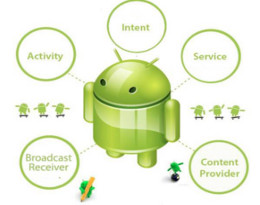
\includegraphics{Components} 
  \caption{Android Components (source: from google search)}
\end{figure}

From the above figure we can see the important components of an android system. These components perform specific actions of an application.
\begin{enumerate}
\item \textbf{Activity} :- these are the panels that we see when we use an application and are basically the GUI part of the application.
\item \textbf{Service} :- these are background processes that can be bound to an application , these are used to perform long or computation intensive operations without holding up the application UI.
\item \textbf{Broadcast Receiver} :- This component listens for outside communications coming from the OS or other apps , For example if the phone receives a SMS an intent is received by an messaging application and a broadcast receiver catches that intent. 
\item \textbf{Content Provider} :- These components are like databases for applications like the SMS inbox on a phone.
\item \textbf{Intent} :- An intent is the message that is passed to the OS or another app.
\end{enumerate}

\begin{figure}
  \centering
 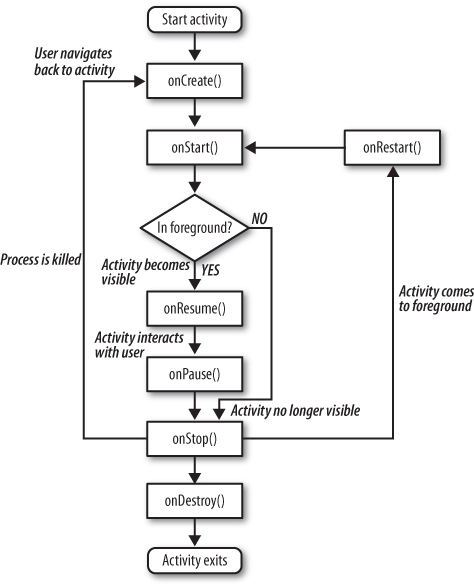
\includegraphics{lifecycle1} 
  \caption{Android Activity Life Cycle (source: from google search)}
\end{figure}

The main tricky part about the android application execution can be seen in the above figure, Where the different entry points namely onCreate(), onStart(), onResume(), onPause(),onStop(),onDestroy() are all executed based on if the app is launched afresh or is minimized etc. The important part here is that there is no main method that goes and executes the application in a clean and sequential manner. An android application when executed first launches an activity designated as its launcher activity which inturn has a callback called OnCreate() which handles the initialization of the application and then based on the input given to that activity any one of the other callback methods may be executed or could move to a different activity that has its own set of callback activities.\\
Imagine a scenario where a person opens an application and as he is using it he receives a phone call which sends the app to the background which call the onPause() callback in the application before minimizing it and then on resuming the application the onResume() callback is executed. Based on the scenario described we can see that the flow of an android application is not sequential and therefore hard to see where there is a leak present or not.  \\

\subsection{Inter procedural control flow graph (ICFG)}
	The main aim of an ICFG[6] is to generate a map or graph of function calls that are called in a program and records the call and return sites. This data structure also contains data pertaining to the data being passed along such procedural calls. This graph is useful to analyze the working of an application as we can see the and exact but abstract flow of data and control through that application.  

\subsection{Taint Analysis}
The previous work in this field was to go though the code and look for an API call that would open an energy consuming resource and continue scanning the code for the statement that will close the said resource but from the previous paragraph we can see that might not always work out as the open and close statements might be present in different places and might not be executed in a good order.  As the combination of user input to the GUI of an app that might completely change the sequence of execution of the code in the application cannot be predicted a dynamic approach of testing the application if the open and closing of resources does occur is not easy as the user might not always use an app in a particular order that will leak information.\\


%	\begin{figure}
  %\centering
 %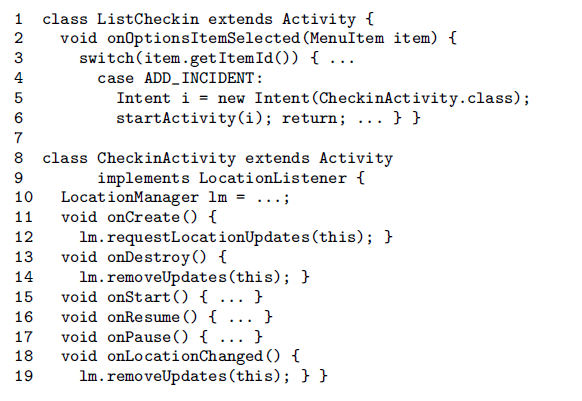
\includegraphics[width=8cm]{probexample} 
  %\caption{Example of usage of GPS API(source: from the paper[1])}
%\end{figure}
The problem that is being solved is to find if an application is leaking private or sensitive data through some sensitive via from an sensitive source.\\
 
\section{Tools In Consideration}
In this work the following three tools are being compared for their performance against two benchmark android security analysis suites namely Droidbench and ICCBench. This comparison will involve running these tools on these benchmark applications and discussing whether the results produced by these tools are accurate.

\begin{itemize}
	\item FlowDroid [3] - Flowdroid utilizes an inter-procedural data flow framework to perform object sensitive analysis and computes a model of the android lifecycle to achieve a fully context sensitive analysis of android applications.
	\item IccTA[1] - Focuses on analyzing one of the more important features of the android system, Inter component communication. IccTA build on top of Flowdroid.
	\item Amandroid [2] - Amandroid creates inter-procedural and data dependence graphs which can be later used to detect sensitive information leaks, but the hallmark of the graphs generated by Amandroid is that any number of security analysis related queries could be run on these graphs. 
\end{itemize}


\subsection{FlowDroid}
	Flowdroid builds an precise model of the android life cycle to perform a fully context sensitive analysis which considers the android application lifecycle and UI widgets.  Flowdroid is the first static taint-analysis system that is fully context, flow, field and object-sensitive while precisely modeling the complete Android lifecycle, including the correct handling of callbacks and user-defined UI widgets within the apps. This design aims to maximize precision and recall, i.e., aims at minimizing the number of missed leaks and false warnings and a particularly novel feature of Flowdroid is the usage of on-demand alias analysis algorithms.\\
	Flowdroid achieves a flow sensitive analysis that is precise by modeling taint analysis within an inter-procedural data flow framework called IFDS[4]. By performing object sensitive analysis we can easily think of a situation where sensitive data is assigned to a heap or an array, in this situation Flowdroid does not flag the entire array or heap as tainted but performs a backward analysis to try and resolve this and figure out if there is actually a leak of sensitive information. This backward analysis also involves going back through already analyzed code to taint aliases of and new variable that holds sensitive data, this is called On-demand alias analysis. \\
\subsection{IccTA}
	One of the defining features of the android system is the message passing system which is known as Inter component communication(ICC), it is responsible for communication between activities and services and receivers and not only within one application but among others installed on a phone as well. This feature is used quite often in all applications as such it is complicated to detect flows that can go in and out of the code base of the application. Li Li et al.[1] focuses on this feature by using the converting the bytecode of an application into Jimple code and collecting all Inter component communication links (APIs) from that code and placing them in an database. All relevent information to ICC calls like URIs, Intents ,Intent filter values etc.. are stored in the database. All of this information on ICC links is obtained by using a tool called Epicc[4] and IC3[5].\\
	In the next step IccTA identifies all possible components from the android manifest file and retrieves the values on intent filters in the applications. Then using all the information gathered in the previous steps IccTA performs taint analysis to find malicious data leaks from a sensitive source to a sensitive sink.\\
\subsection{Amandroid}
	The main contributions of Amandroid to the static analysis of android applications involves the construction of points-to information of all objects and their fields  in an application, using this information Amandroid builds a precise Inter-procedural control flow graph for an application is constructed which could be used to perform a wide variety of analyses with minor changes in the source code of the tool. Amandroid's inter-procedural control flow graph also creates/stores ICC edges and models the android enviroment in such a way that  these flows can be tracked for taint analysis, Amandroid also builds a data dependence graph that could be used to query or detect specific security leaks that are interesting.\\
	Amandroid's approach is broken down into five steps (1) Converting the source code of the application which is in dalvik bytecode to an intermediate form.(2) generate a model of the environment of the android system and limits the model to only those interactions that are applicable to the app.(3) Building of a inter-component data flow graph(IDFG) which is an ICFG with information regarding all data/objects.(4) Building a data dependence graph on top of the inter-component data flow graph to track information flow. (5) Finally using these generated graphs to query is there is sensitive information flow from a source to a sink.\\   


\section{Applications analyzed}
	Summary of applications selected from Droidbench and ICC bench.\\



\begin{itemize}
	\item List of all 10 applications
\end{itemize}
\subsection{Application with sensitive data transferred between activities (ActivityCommunication8)}
\IEEEPARstart{T}{his} app is made up of 3 activities namely OutFlowActivity, InFlowActivity and IsolateActivity. The OutFlowActivity is the main launcher activity of the app and this activity in its onCreate method creates an intent which is directed to an action string , This action string matches the intent filter of the InFlowActivity in the manifest file of the app, The data that is being passed along with the intent that is created is the IMEI number of the phone which is  a sensitive source. When the InFlowActivity is started using this intent it outputs the IMEI  number via a sensitive sink (Log.i()).\\
IsolateActivity here also has the same behavior as InFlowActivity but its intent filter action string is different from InFlowActivity. This might just be in place to test for false alarms.\\
Paths that are interesting in this application
\begin{itemize}
	\item Path 1 :-  Flow from the intent in OutFlowActivity to  the sink in InFlowActivity.
	\item Path 2 :-  Flow from the intent in OutFlowActivity to  the sink in IsolateActivity. Even though there is no flow present in the actual code.
\end{itemize}
In this app the flow that should be detected would be would be the one from the intent in OutFlowActivity to the sink in InFlowActivity. anything else than that would be a false alarm and anything less would be a false negative. 

  

\subsubsection{Analysis of IccTA results}
On running IccTA to analyze this app it reports include 2 paths both Path 1 and Path 2.

Although the Path 1 reported is correct according to the behavior of the app, Path 2 reported is a false alarm as the intent was directed towards the InFlowActivity and not towards the IsolateActivity based on the action string that is provided to the intent in OutFlowActivity. IccTA was unable to distinguish   which activity the intent was directed to hence leading to an false alarm being reported by the tool.

\subsubsection{Analysis of Flowdroid results}
Flowdroid also finds both flows Path 1 and Path 2. The first path that is reported is  a true positive but the second path is false because the intent was never directed to the sink in IsolateActivity.\\


\subsubsection{Analysis of Amandroid results}
Amandroid accurately detected Path 1 , and does not report Path 2 which means that Amandroid performs better than Flowdroid and IccTA. This is a true positive assessment of the application. 


\subsection{Application that sends data to a component not in the manifest (ComponentNotInManifest1)}

\IEEEPARstart{T}{his} app is made up of 4 activities namely OutFlowActivity, InFlowActivity, InFlowinterceptorActivity and IsolateActivity. The OutFlowActivity is the main launcher activity of the app and this activity in its onCreate method creates an intent which is directed to an action string 'InFlowActivity.class' with the data part as the IMEI number of the phone, This app is interesting because only OutFlowActivity and IsolateActvity are the only 2 activities that are declared in the manifest file of the app. The InFlowInterceptorActivity creates a InFlowActivity object and uses this object to intercept that intent that is sent out from the OutFlowActivity which results in InFlowActivvty being started. When the InFlowActivity is started using this intent it outputs the IMEI  number via a sensitive sink (Log.i()).\\
Paths that are interesting in this application
\begin{itemize}
	\item Path 1 :-  Flow from the intent in OutFlowActivity to the sink in InFlowActivity.
	\item Path 2 :-  Flow from the intent in OutFlowActivity to the sink in IsolateActivity. Even though there is no flow present in the actual code.
\end{itemize}


IsolateActivity here also has the same behavior as InFlowActivity but its intent filter action string is different from InFlowActivity. This might just be in place to test for false alarms.\\


In this app the flow that should be detected would be would be the one from the intent in OutFlowActivity to the sink in InFlowActivity. anything else than that would be a false alarm and anything less would be a false negative. 

  

\subsubsection{Analysis of IccTA results}
The tools reports only 1 path which is Path 2 and Path 2 this is obviously a false alarm as the intent was never directed to the IsolateActivity in the first place.\\
The real flow that is actually relevant, which is Path 1, is missed completely which also counts as a false negative.


\subsubsection{Analysis of Flowdroid results}
Flowdroid also fails to detect Path 1 which is a false negative. and detects the same non-existent Path 2 which is a false positive.

\subsubsection{Analysis of Amandroid results}
Amandroid detects all the sources and sinks present in the application but fails to find any flow present in the application as such this is a False negative  for Path 1 and a True negative for Path 2.


\subsection{Sensitive data leak via dynamically registered receiver (BroadcastTaintLeak1)}
% The very first letter is a 2 line initial drop letter followed
% by the rest of the first word in caps.
% 
% form to use if the first word consists of a single letter:
% \IEEEPARstart{A}{demo} file is ....
% 
% form to use if you need the single drop letter followed by
% normal text (unknown if ever used by IEEE):
% \IEEEPARstart{A}{}demo file is ....
% 
% Some journals put the first two words in caps:
% \IEEEPARstart{T}{his demo} file is ....
% 
% Here we have the typical use of a "T" for an initial drop letter
% and "HIS" in caps to complete the first word.
\IEEEPARstart{T}{his} app is made up of 1 activity which is BroadcastTest. A broadcast receiver is registered in this activity and an intent with a sensitive source (IMEI number) is used to send to this broadcast, in the onreceive method of this receiver there is a sensitive sink (Log.i()) which is used to output the data in the intent sent to the receiver. it should be noted that the broadcast receiver is not defined in the manifest file of the app.\\
Path that are interesting in this application
\begin{itemize}
	\item Path 1 :-  Flow from the intent in BroadcastTest activity to the sink in registered receiver in that Activity.
\end{itemize}

In this app the flow that should be detected would be Path 1. anything else than that would be a false alarm and anything less would be a false negative. 

  

\subsubsection{Analysis of IccTA results}
The tool reports that it has found 2 sources and  1 sink , but does not report ant flow from one to another and give no results, IccTA was unable to detect this leak at all with no flow from source to sink detected.\\
What is interesting is that IccTA has detected 2 sources when there is clearly only 1 in the app.


\subsubsection{Analysis of Flowdroid results}
Flowdroid also fails to detect Path 1. \\
Flowdroid fails to detect anything wrong with the application so this analysis is a false negative.\\

\subsubsection{Analysis of Amandroid results}
Amandroid was able to find Path 1. This is better than both Flowdroid and IccTA as both those tools were unable to detect anything wrong with this application. Amandroid gives a true positive assessment of this application.


\subsection{Sensitive data leak via a messenger service (ServiceCommunication1)}
% The very first letter is a 2 line initial drop letter followed
% by the rest of the first word in caps.
% 
% form to use if the first word consists of a single letter:
% \IEEEPARstart{A}{demo} file is ....
% 
% form to use if you need the single drop letter followed by
% normal text (unknown if ever used by IEEE):
% \IEEEPARstart{A}{}demo file is ....
% 
% Some journals put the first two words in caps:
% \IEEEPARstart{T}{his demo} file is ....
% 
% Here we have the typical use of a "T" for an initial drop letter
% and "HIS" in caps to complete the first word.
\IEEEPARstart{T}{his} app is made up of 1 activity which is ActivityMessenger and 1 service called MessengerService. This app uses a binded messenger service to pass /send sensitive data from the ActivityMessenger to the MessengerService which has a sensitive sink to get the data being sent from the activity\\

Path that are interesting in this application
\begin{itemize}
	\item Path 1 :-  Flow from the one from the service.send() method in the activity t the sink the handleMessage() method in the service in the app.
\end{itemize}

In this app the flow that should be detected would be Path 1. anything else than that would be a false alarm and anything less would be a false negative. \\

  

\subsubsection{Analysis of IccTA results}
The tool reports that it has found no sinks and then it aborts the analysis as there are no sinks , this is quite intelligent as if there are no sensitive sinks there would be no need to perform any analysis as nothing would leak out. \\
But there is a sink present in the app but IccTa fails to detect anything wrong with the app. Which means this is a false negative.

\subsubsection{Analysis of Flowdroid results}
Flowdroid also fails to detect Path 1. It also fails to indicate any reason why there is no result unlike IccTa which indicated that there are no sinks. \\
Flowdroid fails to detect anything wrong with the application so this analysis is a false negative.\\

\subsubsection{Analysis of Amandroid results}
Amandroid also fails to detect Path 1. Amandroid also fails to detect anything , as it does not report either sensitive sources or sinks.\\
Amandroid fails to detect anything wrong with this application so the analysis is a false negative.\\


\subsection{Sensitive data leak via an intent (IntentSink2)}
% The very first letter is a 2 line initial drop letter followed
% by the rest of the first word in caps.
% 
% form to use if the first word consists of a single letter:
% \IEEEPARstart{A}{demo} file is ....
% 
% form to use if you need the single drop letter followed by
% normal text (unknown if ever used by IEEE):
% \IEEEPARstart{A}{}demo file is ....
% 
% Some journals put the first two words in caps:
% \IEEEPARstart{T}{his demo} file is ....
% 
% Here we have the typical use of a "T" for an initial drop letter
% and "HIS" in caps to complete the first word.
\IEEEPARstart{T}{his} app is made up of 1 activity which is IntentSink2 . This app has a text field in th UI of the app in which a intent filter action string can be input into, which on pressing a button will send a intent with its destination as the string entered in the text field with some sensitive data(IMEI number here).\\

Path that are interesting in this application
\begin{itemize}
	\item Path 1 :-  Flow from the one from the intent in the activity to the sink the startActivity()  in the activity.
\end{itemize}


In this app the flow that should be detected would be Path 1. anything else than that would be a false alarm and anything less would be a false negative. \\

  

\subsubsection{Analysis of IccTA results}
The tool reports that it has found 3 sources and 1 sink but is unable to find any flow among them, IccTA was not able to find a path that leads to any information leaking,\\
Again what is interesting is that IccTA has found 3 sources but there is only 1 in the app.

\subsubsection{Analysis of Flowdroid results}
This tool accurately found Path 1.\\
This analysis is a true positive assessment of the application.\\

\subsubsection{Analysis of Amandroid results}
Amandroid fails to detect Path 1. Amandroid also fails to identify any sources or sinks in the  application.\\ Since amandroid fails to find anything wrong with the application the analysis is a false negative assessment of the application.

\subsection{Sensitive data leak via the Activity life cycle  callback methods (ActivityLifecycle4)}
% The very first letter is a 2 line initial drop letter followed
% by the rest of the first word in caps.
% 
% form to use if the first word consists of a single letter:
% \IEEEPARstart{A}{demo} file is ....
% 
% form to use if you need the single drop letter followed by
% normal text (unknown if ever used by IEEE):
% \IEEEPARstart{A}{}demo file is ....
% 
% Some journals put the first two words in caps:
% \IEEEPARstart{T}{his demo} file is ....
% 
% Here we have the typical use of a "T" for an initial drop letter
% and "HIS" in caps to complete the first word.
\IEEEPARstart{T}{his} app is simple in that when the application is paused it sends an SMS to a attackers phone number with the victims phones IMEI number as the message and the IMEI number is fetched when the application is resumed. The SMS is sent without the victim knowing ( i.e. silently sent).\\

Path that are interesting in this application
\begin{itemize}
	\item Path 1 :-  Flow  from the sensitive source API call in the onResume() callback in the main activity to the onPause() callback's sensitive sink .
\end{itemize}

The flow that should be detected should be Path 1 reporting any other flows would be a false alarm and anything less would be a false negative.\\
  

\subsubsection{Analysis of IccTA results}
IccTA accurately found Path 1.\\
This analysis is a true positive assessment of the application.\\
\subsubsection{Analysis of Flowdroid results}
This tool accurately found Path 1.\\
This analysis is a true positive assessment of the application.\\

\subsubsection{Analysis of Amandroid results}
Amandroid accurately finds Path 1.\\
This analysis is a true positive assessment of the application.\\

\subsection{Sensitive data leak via ordering of activity callback methods (EventOrdering1)}
% The very first letter is a 2 line initial drop letter followed
% by the rest of the first word in caps.
% 
% form to use if the first word consists of a single letter:
% \IEEEPARstart{A}{demo} file is ....
% 
% form to use if you need the single drop letter followed by
% normal text (unknown if ever used by IEEE):
% \IEEEPARstart{A}{}demo file is ....
% 
% Some journals put the first two words in caps:
% \IEEEPARstart{T}{his demo} file is ....
% 
% Here we have the typical use of a "T" for an initial drop letter
% and "HIS" in caps to complete the first word.
\IEEEPARstart{T}{his} app is interesting in the fact that the sensitive sink and the sensitive source are called in the same callback function but the sink is called before the source. But since callback functions in an android applications can be run at any point any number of times based on user actions, when that call back function is called again (in this case onLowMemory()) the sink now has the data already available.\\

Path that are interesting in this application
\begin{itemize}
	\item Path 1 :-  Flow from the flow in the onLowMemory callback to the sink in the onLowMemory callback.
\end{itemize}

There is 1 flow in this app which is Path 1 reporting any other flows would be a false alarm and anything less would be a false negative. 

\subsubsection{Analysis of IccTA results}
IccTA tool accurately found Path 1 so this is a true positive assessment of this application.\\
\subsubsection{Analysis of Flowdroid results}
This tool accurately found Path 1 so this is a true positive assessment of this application.\\

\subsubsection{Analysis of Amandroid results}
Amandroid could also find Path 1.\\ Amandroid gives a true positive assessment of this application.

\subsection{Sensitive data passed between multiple components and then leaked (AndroidSpecific\_PrivateDataLeak3)}
% The very first letter is a 2 line initial drop letter followed
% by the rest of the first word in caps.
% 
% form to use if the first word consists of a single letter:
% \IEEEPARstart{A}{demo} file is ....
% 
% form to use if you need the single drop letter followed by
% normal text (unknown if ever used by IEEE):
% \IEEEPARstart{A}{}demo file is ....
% 
% Some journals put the first two words in caps:
% \IEEEPARstart{T}{his demo} file is ....
% 
% Here we have the typical use of a "T" for an initial drop letter
% and "HIS" in caps to complete the first word.
\IEEEPARstart{T}{his} app is from the ICC bench suite of applications for testing static analysis of android applications. In this app the password field from a form on the main activity on being entered is passed from the MainActivity onto another activity called FooActivity then on another activity called BarActivty where it is leaked out through a sensitive sink.

Path that are interesting in this application
\begin{itemize}
	\item Path 1 :-  Flow of sensitive data from the MainActivity via FooActivity and finally to the sink present in BarActivity.
\end{itemize}

 The flow that should be detected should include all there activities any other flows would be a false alarm and anything less would be a false negative. 

\subsubsection{Analysis of IccTA results}
IccTA tool accurately found Path 1 so this is a true positive assessment of this application.\\
\subsubsection{Analysis of Flowdroid results}
This tool accurately found Path 1 so this is a true positive assessment of this application.\\

\subsubsection{Analysis of Amandroid results}
Amandroid accurately found Path 1 .Since amandroid was able to track this flow of sensitive data this is a true positive assessment of this application.\\

\subsection{Application with sensitive data in an object like an array or heap (FieldAndObjectSensitivity\_FieldFlowSensitivity1)}
% The very first letter is a 2 line initial drop letter followed
% by the rest of the first word in caps.
% 
% form to use if the first word consists of a single letter:
% \IEEEPARstart{A}{demo} file is ....
% 
% form to use if you need the single drop letter followed by
% normal text (unknown if ever used by IEEE):
% \IEEEPARstart{A}{}demo file is ....
% 
% Some journals put the first two words in caps:
% \IEEEPARstart{T}{his demo} file is ....
% 
% Here we have the typical use of a "T" for an initial drop letter
% and "HIS" in caps to complete the first word.
\IEEEPARstart{T}{his} app is from the ICC bench suite of applications for testing static analysis of android applications. This application has 2 activities MainActivity and FooActivity , there is another java class called Data is used to store and retrieve 2 strings, In the MainActivty a string ``data''  is stored using this Data class object, then another string is stored into this object which is the IMEI number of the phone which is a sensitive source. This object is put into an Intent and sent to the FooActivity. In this FooActivity the data object is retried from the intent and the first string which is harmless is put into a sensitive sink (Log.i()) ,whereas the sensitive data in the second string is left undisturbed. So the only relevant flows that should be reported is from the OnCreate method in MainActivity to the Intent flowing out of it, Reporting anyother flows would be a false positive and anything less would be a false negative.

Path that are interesting in this application
\begin{itemize}
	\item Path 1 :-  Flow of sensitive data from the MainActivity to the intent created in MainActivity.
\end{itemize}

\subsubsection{Analysis of IccTA results}
IccTA accurately reports only Path 1 and does not report anything else which is a true positive assessment of the application.
\subsubsection{Analysis of Flowdroid results}
Flowdroid accurately reports only Path 1 and does not report anything else which is a true positive assessment of the application.
\subsubsection{Analysis of Amandroid results}
Amandroid accurately reports  Path 1 but also reports the flow into the  Log.i() in FooActivty which is not a true flow as the data being leaked out via the Log.i() is not sensitive data. So Amandroid raises a false positive alarm after analyzing this application.


\subsection{Sensitive data leak via registered receiver  (DynRegister2)}
% The very first letter is a 2 line initial drop letter followed
% by the rest of the first word in caps.
% 
% form to use if the first word consists of a single letter:
% \IEEEPARstart{A}{demo} file is ....
% 
% form to use if you need the single drop letter followed by
% normal text (unknown if ever used by IEEE):
% \IEEEPARstart{A}{}demo file is ....
% 
% Some journals put the first two words in caps:
% \IEEEPARstart{T}{his demo} file is ....
% 
% Here we have the typical use of a "T" for an initial drop letter
% and "HIS" in caps to complete the first word.
\IEEEPARstart{T}{his} app is from the ICC bench suite of applications for testing static analysis of android applications. This application has 1 activity called MainActivity and a broadcast receiver that is registered in the activity. The main difference between this application and the BroadcastTaintLeak1 that we analyzed earlier is that the registered receiver's intent filter parameter is provided a string builder object with the intent filter string as data as opposed to just providing a standard string.\\
The flow that needs to be detected in this application is the flow of sensitive data from MainActivity to the sink in the broadcast receiver. Reporting any thing else would be a false positive and anything less would be a false negative.\\
Path that are interesting in this application
\begin{itemize}
	\item Path 1 :-  Flow of sensitive data from the MainActivity to the sink in the broadcast receiver.
\end{itemize}

\subsubsection{Analysis of IccTA results}
IccTA was not able to detect Path 1, as such this is a false negative assessment of the application. 

\subsubsection{Analysis of Flowdroid results}
Flowdroid was not able to detect Path 1, as such this is a false negative assessment of the application. 
\subsubsection{Analysis of Amandroid results}
Amandroid accurately reports  Path 1, as such this is a true positive assessment of the application.
   
\newpage
\newcommand{\specialcell}[2][c]{%
  \begin{tabular}[#1]{@{}c@{}}#2\end{tabular}}
\section{Results Table}
\begin{table}[h!]
  \centering
  \caption{Table comparing results of analysis of IccTA on Droidbench Apps on Intel i5  with 8GB Memory}
  \label{tab:table1}
   \resizebox{\textwidth}{!}{
  \begin{tabular}{|l|l|l|l  | l | l |l| }
  \hline
    App Name & Ground Truth &Relevent Flows Detected& Flow  Analysis & Percentage of accuracy & Time complexity  \\
    \hline 
    ActivityCommunication8 & OutFlowActivty to InflowActivty & \specialcell[l]{1.)OutFlowActivty to InflowActivty\\2.)OutFlowActivty to IsolateActivty}   & \specialcell[l]{1.)True Positive\\2.)False Positive} & 50\% & 14 sec \\
    \hline 
    ComponentNotInManifest1 & OutFlowActivty to InflowActivty& \specialcell[l]{1.)OutFlowActivty to InflowActivty\\2.)OutFlowActivty to IsolateActivty}  &\specialcell[l]{1.)False negative\\2.)False Positive} & 0\% & 8 sec   \\	    
     \hline 
    BroadcastTaintLeak1 & BroadcastTest activity to receiver&BroadcastTest activity to receiver & False negative & 0\% & 8 sec \\
   \hline 
   ServiceCommunicationa &ActivtyMessenger activity to MessengerService service & ActivtyMessenger activity to MessengerService service   & False Negative & 0\% & 12 sec \\
   \hline 
    IntentSink2 & The intent in startActivity() &The intent in startActivity()  & False negative & 0\% & 8 sec\\
  \hline
   ActivityLifeCycle4 &  onResume() callback to onPause() callback  & onResume() callback to onPause() callback  &  True Positive & 100\% & 10 sec\\
  \hline
    EventOrdering1 &  onLowMemory() callback with sink called before source  & onLowMemory() callback with sink called before source  &  True Positive & 100\% & 10 sec\\
  \hline
    AndroidSpecific\_PrivateDataLeak3 & MainActivity to FooActivity to BarActivity & MainActivity to FooActivity to BarActivity   & True Positive & 100\% & 14 sec\\
  \hline
  FieldAndObjectSensitivity\_FieldFlowSensitivity1 &  The intent in MainActivity &The intent in MainActivity & True Positive & 100\% & 14 sec\\
  \hline
  DynRegister2  & Flow from MainActivity to Receiver & No Flow Detected & True Positive & 0\% & 14 sec\\
  \hline
  \end{tabular}}
\end{table}


\section{Results Table}

\begin{table}[h!]
  \centering
  \caption{Table comparing results of analysis of FlowDorid on Droidbench/ICCBench Apps on Ohio Super Computer(OSC)  with 128GB Memory}
  \label{tab:table2}
   \resizebox{\textwidth}{!}{
  \begin{tabular}{|l|l|l|l  | l | l |l| }
  \hline
    App Name & Ground Truth & Relevent Flows Detected & Flow  Analysis & Percentage of accuracy & Time complexity  \\
    \hline 
    ActivityCommunication8 & OutFlowActivty to InflowActivty &  \specialcell[l]{1.)OutFlowActivty to InflowActivty\\2.)OutFlowActivty to IsolateActivty}   & \specialcell[l]{1.)True Positive\\2.)False Positive} & 50\% & 12 sec \\
    \hline 
    ComponentNotInManifest1 & OutFlowActivty to InflowActivty & \specialcell[l]{OutFlowActivty to IsolateActivty}  &\specialcell[l]{False Positive} & 0\% & 8 sec   \\	    
     \hline 
    BroadcastTaintLeak1 & BroadcastTest activity to receiver & No Flow Detected& False negative & 0\% & 10 sec \\
   \hline 
   ServiceCommunicationa &  ActivtyMessenger activity to MessengerService service   &No Flow detected & False negative & 0\% & 12 sec \\
   \hline 
    IntentSink2 &  The intent in startActivity()  &The intent in startActivity()  & True Positive & 100\% & 8 sec\\
  \hline
    ActivityLifeCycle4 &  onResume() callback to onPause() callback  & onResume() callback to onPause() callback  &  True Positive & 100\% & 10 sec\\
  \hline
    EventOrdering1 &  onLowMemory() callback with sink called before source  & onLowMemory() callback with sink called before source  &  True Positive & 100\% & 8 sec\\
  \hline
    AndroidSpecific\_PrivateDataLeak3 & MainActivity to FooActivity to BarActivity & MainActivity to FooActivity to BarActivity   & True Positive & 100\% & 13 sec\\
  \hline
  FieldAndObjectSensitivity\_FieldFlowSensitivity1 &  The intent in MainActivity &The intent in MainActivity & True Positive & 100\% & 13 sec\\
  \hline
  DynRegister2  & Flow from MainActivity to Receiver & No Flow Detected & True Positive & 0\% & 13 sec\\
  \hline
  \end{tabular}}
\end{table}


\section{Results Table}

\begin{table}[h!]
  \centering
  \caption{Table comparing results of analysis of Amandroid on Droidbench/ICCBench Apps on Ohio Super Computer(OSC)  with 128GB Memory}
  \label{tab:table3}
   \resizebox{\textwidth}{!}{
  \begin{tabular}{|l|l|l|l  | l | l |l| }
  \hline
    App Name & Ground Truth & Relevent Flows Detected & Flow  Analysis & Percentage of accuracy & Time complexity  \\
    \hline 
    ActivityCommunication8 & OutFlowActivty to InflowActivty &  \specialcell[l]{1.)OutFlowActivty to InflowActivty\\2.)OutFlowActivty to IsolateActivty}   & \specialcell[l]{1.)True Positive\\2.)True Negative} & 100\% & 12 sec \\
    \hline 
    ComponentNotInManifest1 & OutFlowActivty to InflowActivty & \specialcell[l]{OutFlowActivty to IsolateActivty}  &\specialcell[l]{False Positive} & 0\% & 8 sec   \\	    
     \hline 
    BroadcastTaintLeak1 & BroadcastTest activity to receiver & BroadcastTest activity to receiver & True positive & 100\% & 10 sec \\
   \hline 
   ServiceCommunicationa &  ActivtyMessenger activity to MessengerService service   &No Flow detected & 0\% & 12 sec \\
   \hline 
    IntentSink2 &  The intent in startActivity()  &No Flow Detected  & False Negative & 0\% & 8 sec\\
  \hline
    ActivityLifeCycle4 &  onResume() callback to onPause() callback  & onResume() callback to onPause() callback  &  True Positive & 100\% & 10 sec\\
  \hline
    EventOrdering1 &  onLowMemory() callback with sink called before source  & onLowMemory() callback with sink called before source  &  True Positive & 100\% & 8 sec\\
  \hline
    AndroidSpecific\_PrivateDataLeak3 & MainActivity to FooActivity to BarActivity & MainActivity to FooActivity to BarActivity   & True Positive & 100\% & 13 sec\\
  \hline
  FieldAndObjectSensitivity\_FieldFlowSensitivity1 &  The intent in MainActivity & The intent in MainActivity and flow into the Log.i() in FooActivity & True Positive & 50\% & 13 sec\\
  \hline
  DynRegister2  & Flow from MainActivity to Receiver & Flow from MainActivity to Receiver & True Positive & 100\% & 13 sec\\
  \hline
  \end{tabular}}
\end{table}


\newpage
asa
\newpage
%\begin{sidewaystable}
   % \centering
\begin{table}
  \caption{Table comparing results of analysis of FlowDorid , Amandroid on Droidbench/ICCBench Apps on Ohio Super Computer(OSC)  with 128GB Memory}
  \label{tab:table3}
  \resizebox{\textwidth}{!}{
  \begin{tabular}{|l|l|l|l  | l | l | l|}
  \hline
    App Name  & Flow  Analysis Accuracy of IccTA & Flow Analysis Accuracy of Flowdroid & Flow Analysis Accuracy of Amandroid \\
    \hline 
    ActivityCommunication8 & 50\%& 50\% & 100\%  \\
    \hline 
    ComponentNotInManifest1 &0\%&0\% & 0\%    \\	    
     \hline 
    BroadcastTaintLeak1   & 0\%& 0\% & 100\% \\
   \hline 
   ServiceCommunication1   & 0\% & 0\% & 0\% \\
   \hline 
    IntentSink2  & 0\%& 100\% & 0\%\\
  \hline
    ActivityLifeCycle4  & 100\%& 100\% & 100\% \\
  \hline
    EventOrdering1   & 100\%& 100\% &100\% \\
  \hline
    AndroidSpecific\_PrivateDataLeak3  & 100\%& 100\% & 100\%\\
  \hline
   FieldAndObjectSensitivity\_FieldFlowSensitivity1  & 100\% & 100\% & 50\%\\
  \hline
   DynRegister2  & 0\% & 0\% & 100\%\\
  \hline
  \end{tabular}
}
\end{table}
%\end{sidewaystable}




% Can use something like this to put references on a page
% by themselves when using endfloat and the captionsoff option.
\ifCLASSOPTIONcaptionsoff
  \newpage
\fi



% trigger a \newpage just before the given reference
% number - used to balance the columns on the last page
% adjust value as needed - may need to be readjusted if
% the document is modified later
%\IEEEtriggeratref{8}
% The "triggered" command can be changed if desired:
%\IEEEtriggercmd{\enlargethispage{-5in}}

% references section

% can use a bibliography generated by BibTeX as a .bbl file
% BibTeX documentation can be easily obtained at:
% http://www.ctan.org/tex-archive/biblio/bibtex/contrib/doc/
% The IEEEtran BibTeX style support page is at:
% http://www.michaelshell.org/tex/ieeetran/bibtex/
%\bibliographystyle{IEEEtran}
% argument is your BibTeX string definitions and bibliography database(s)
%\bibliography{IEEEabrv,../bib/paper}
%
% <OR> manually copy in the resultant .bbl file
% set second argument of \begin to the number of references
% (used to reserve space for the reference number labels box)

\newpage
\begin{thebibliography}{1}

\bibitem{1}
Li, Li, et al. "Iccta: Detecting inter-component privacy leaks in android apps." Proceedings of the 37th International Conference on Software Engineering-Volume 1. IEEE Press, 2015.
\bibitem{2}
Wei, Fengguo, Sankardas Roy, and Xinming Ou. "Amandroid: A precise and general inter-component data flow analysis framework for security vetting of android apps." Proceedings of the 2014 ACM SIGSAC Conference on Computer and Communications Security. ACM, 2014.
\bibitem{3}
Arzt, Steven, et al. "Flowdroid: Precise context, flow, field, object-sensitive and lifecycle-aware taint analysis for android apps." ACM SIGPLAN Notices 49.6 (2014): 259-269.

 \bibitem{4}
 D. Octeau, P. McDaniel, S. Jha, A. Bartel, E. Bodden, J. Klein, and
Y. Le Traon. Effective inter-component communication mapping in
android with epicc: An essential step towards holistic security analysis.
In Proceedings of the 22nd USENIX Security Symposium, 2013
 
\bibitem{5}
D. Octeau, D. Luchaup, M. Dering, S. Jha, and P. McDaniel. Composite
constant propagation: Application to android inter-component communication
analysis. In Proceedings of the 37th International Conference
on Software Engineering (ICSE), 2015.
\bibitem{6}
M. Sharir and A. Pnueli. Two approaches to interprocedural data
flow analysis. In S. Muchnick and N. Jones, editors, Program Flow
Analysis: Theory and Applications, pages 189–234. Prentice Hall,
1981.
\end{thebibliography}



% You can push biographies down or up by placing
% a \vfill before or after them. The appropriate
% use of \vfill depends on what kind of text is
% on the last page and whether or not the columns
% are being equalized.

%\vfill

% Can be used to pull up biographies so that the bottom of the last one
% is flush with the other column.
%\enlargethispage{-5in}



% that's all folks
\end{document}


